\chapter{Исследовательский раздел}

\section{Исследоваеие скорости работы алгоритма}

Для исследования скоростных характеристик был использован компьютер на базе процессора Intel Core i5-4570, содержащий 8 гигабайт оперативной памяти. Стоит учесть, что модуль тестирования запускался с жестокго диска под операционной системой Ubuntu 16.04. Жесткий диск имел среднюю скорость передачи данных при чтении 85,3 Мбайт/с, а время доступа — 16,3 мс. 

\begin{figure}[ht!]
	\centering{ 
		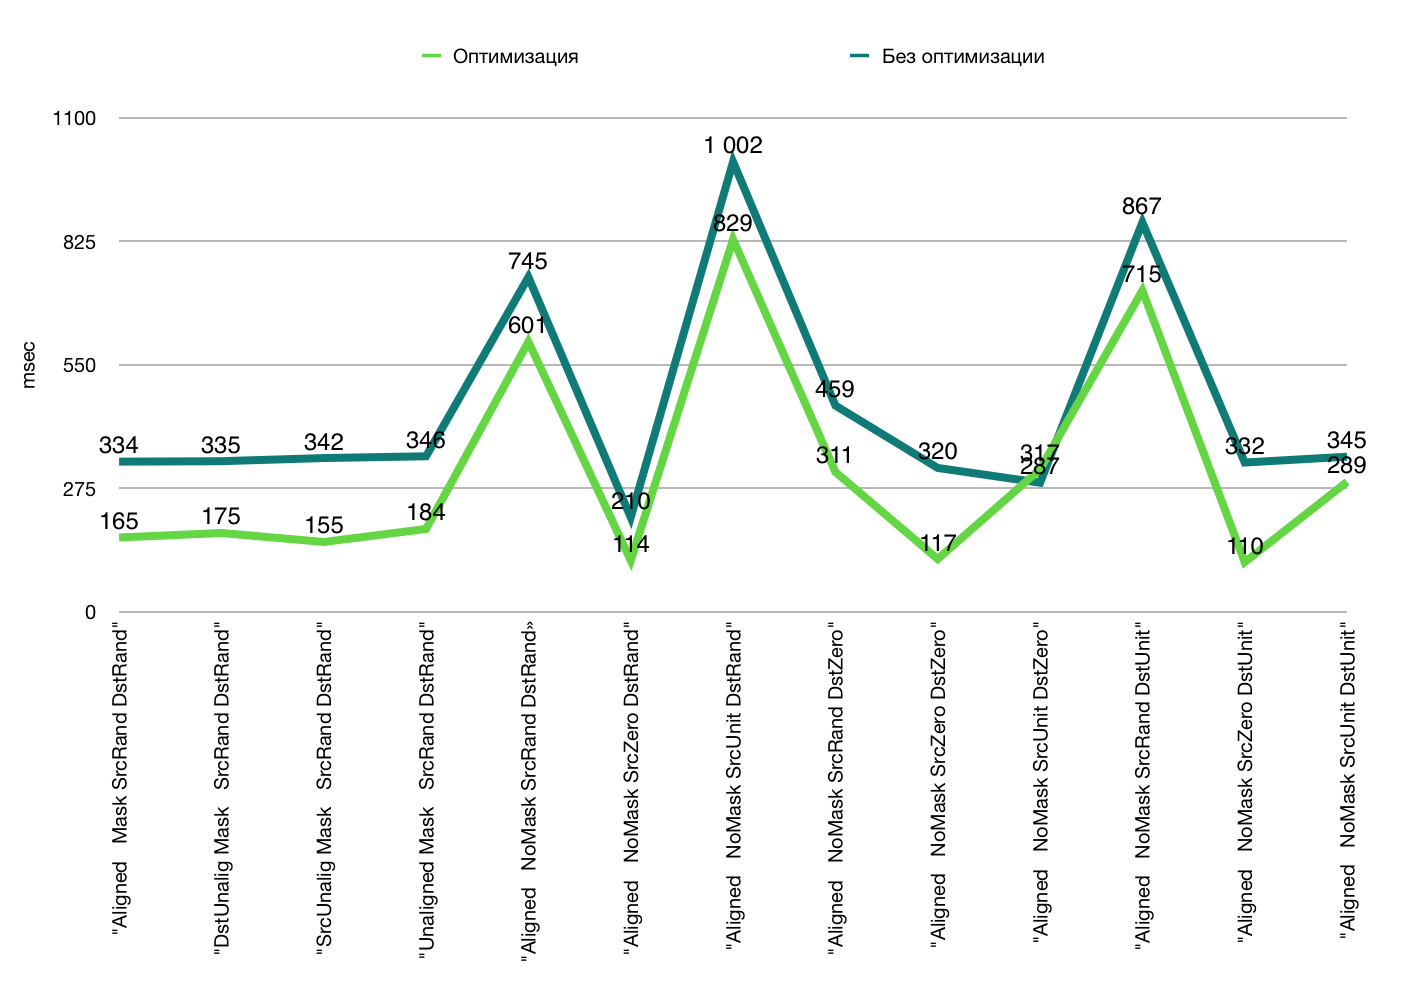
\includegraphics[width=1\textwidth]{img/9.png}
		\caption{Графих средней скорости работы}}
\end{figure}

Пояснение кодировку имени тестов. 
\begin{enumerate}
\item Aligned -- тесты с выровнеными данными.
\item Mask -- тесты с использованием маски.
\item SrcRand, SrcZero, SrcUnit -- исходное изображение заполненно соответственно случайными пикселями, черными и одинаковыми. Dst аналогично.
\end{enumerate}

На рисунке 4.1 видим, что нам удалось добиться ускорения работы программу почти в два раза.
%%% Local Variables:
%%% mode: latex
%%% TeX-master: "rpz"
%%% End:
